\documentclass{article}
\usepackage{amsmath,amsfonts,amsthm,amssymb,amsopn,bm}
\usepackage[margin=.9in]{geometry}
\usepackage{graphicx}
\usepackage{url}
\usepackage[usenames,dvipsnames]{color}
\usepackage{fancyhdr}
\usepackage{multirow}
\usepackage{listings}
\usepackage{hyperref}

\definecolor{keywords}{RGB}{255,0,90}
\definecolor{comments}{RGB}{0,0,113}
\definecolor{red}{RGB}{160,0,0}
\definecolor{green}{RGB}{0,150,0}
 
\lstset{language=Python, 
        basicstyle=\ttfamily\tiny, 
        keywordstyle=\color{keywords},
        commentstyle=\color{comments},
        stringstyle=\color{red},
        showstringspaces=false}

\newcommand{\argmax}{\arg\!\max}
\newcommand{\argmin}{\arg\!\min}
\newcommand{\field}[1]{\mathbb{#1}}
\newcommand{\1}{\mathbf{1}}
\newcommand{\E}{\mathbb{E}} 
\renewcommand{\P}{\mathbb{P}}
\newcommand{\N}{\mathcal{N}} % NormalDist
\newcommand{\R}{\field{R}} % real domain
% \newcommand{\C}{\field{C}} % complex domain
\newcommand{\F}{\field{F}} % functional domain
\newcommand{\T}{^{\textrm T}} % transpose
\def\diag{\text{diag}}

%% operator in linear algebra, functional analysis
\newcommand{\inner}[2]{#1\cdot #2}
\newcommand{\norm}[1]{\left\|#1\right\|}
\newcommand{\twonorm}[1]{\|#1\|_2^2}
% operator in functios, maps such as M: domain1 --> domain 2
\newcommand{\Map}[1]{\mathcal{#1}}
\renewcommand{\theenumi}{\alph{enumi}} 

\newcommand{\Perp}{\perp \! \! \! \perp}

\newcommand\independent{\protect\mathpalette{\protect\independenT}{\perp}}
\def\independenT#1#2{\mathrel{\rlap{$#1#2$}\mkern2mu{#1#2}}}
\newcommand{\vct}[1]{\boldsymbol{#1}} % vector
\newcommand{\mat}[1]{\boldsymbol{#1}} % matrix
\newcommand{\cst}[1]{\mathsf{#1}} % constant
\newcommand{\ProbOpr}[1]{\mathbb{#1}}
\newcommand{\points}[1]{\small\textcolor{magenta}{\emph{[#1 points]}} \normalsize}
\date{{}}

\setlength\parindent{0px}

\begin{document}
\title{Homework \#1 B}
\author{\normalsize{Spring 2020, CSE 446/546: Machine Learning}\\
\normalsize{Dino Bektesevic}}
\maketitle

\section*{B2}
Use just the definitions above and let $||\cdot||$ be a norm.
\begin{enumerate}
    \item \points{3} Show that $f(x)=||x||$ is a convex function. \\
    See A.1. problem, this follows directly from the definition of a norm's absolute scalability and triangle inequality. Start from definition of a convex function $f(\lambda x + (1-\lambda)y) \leq \lambda f(x) + (1-\lambda)f(y) \forall\lambda\in[0,1]$ and for any $x,y\in\mathcal{D}$ where $\mathcal{D}$ is a non-empty domain of f and f is our norm:
    \begin{align*}
        ||\lambda x + (1-\lambda)y|| &\leq ||\lambda x|| + ||(1-\lambda)y|| \\
        ||\lambda x + (1-\lambda)y|| &\leq \lambda ||x|| + (1-\lambda)||y||
    \end{align*}
    
    \item \points{3} Show that ${x\in\R^n : ||x||\leq 1}$ is a convex set. \\
    This one is more logically involved than previous problem but the same approach applies. For two points $x$, $y$ from the functions codomain ($[0,1]$) we must show that the expression $\lambda x + (1-\lambda)y)$ is also in the codomain. Assume that $x,y \in [0,1]$ and $||x||<||y||$ and apply the definition : 
    \begin{align*}
        ||\lambda x + (1-\lambda)y|| &\leq  \lambda ||x|| + (1-\lambda)||y|| <  \lambda ||x|| + (1-\lambda)||x|| \\
        ||\lambda x + (1-\lambda)y|| &< \lambda ||x|| + ||x||-\lambda||x|| = ||x|| \leq 1\\
        ||\lambda x + (1-\lambda)y|| &< 1 
    \end{align*}
    
    
    \item \points{2} Draw a picture of the set ${(x1,x2) : g(x_1,x_2)\leq 4}$ where $g(x1,x2) =(|x_1|^{1/2} + |x_2|^{1/2})^2$.(This is the function considered in 1b above specialized to $n=2$.)  We know $g$ is not a norm. Is the defined set convex? Why not?
    This is also a partiall answer to question in A.0. Regularizer "spikiness" produces sparser weights. 
    \begin{figure}
        \centering
        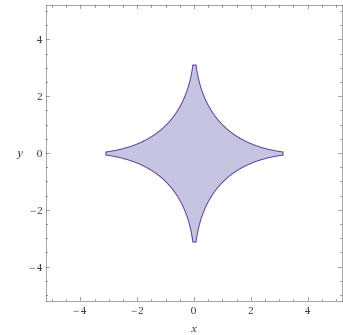
\includegraphics{HW2/HW2_plots/convexSetPlot.png}
        \caption{Caption}
        \label{fig:my_label}
    \end{figure}{}
    
\end{enumerate} 

Context:  It is a fact that a function $f$ defined over a set $A\subseteq R^n$ is convex if and only if the set ${(x,z)\in\R^{n+1}:z\geq f(x), x\in A}$ is convex.  Draw a picture of this for yourself to be sure you understand it.


\end{document}
